\chapter{Classification}

\section{Hardware resources}
Multiple servers, provided by the cognitive system lab, were used. One of the provided servers is optimized for storing large amounts of data and was therefore used to store the histories and the results from the models during training while the other servers focus on computing power and were used to execute that training and evaluation. Mainly two servers were used for the training. One has the hardware specification shown in table \todo{ref} and the other one those shown in table \todo{ref}. 


\begin{table}[H]
	\centering
	\caption{add caption}
	\resizebox{\columnwidth}{!}{%
		\begin{tabular}{l|ll}
			Component & Model & Additional details                   \\
			\hline
			Processing Unit    & Intel® Xeon® Gold Prozessor 5218      & 64 logical cores, \\
								&									& turbo boosts to 3,90 GHz \\
			System Memory      & -                      	           & 377 GB          \\
			Grafics            & 2 x NVIDIA RTX 2080 ti        		   & 11 GB graphics memory                   
		\end{tabular}
	}
\end{table}

\begin{table}[H]
	\centering
	\caption{add caption}
	\resizebox{\columnwidth}{!}{%
		\begin{tabular}{l|ll}
			Component & Model & Additional details                   \\
			\hline
			Processing Unit    & Intel® Xeon® Prozessor E5-2650 v4     & 24 logical cores, \\
			&									& turbo boosts to 2,90 GHz \\
			System Memory      & -                      	           & 252 GB          \\
			Grafics            & NVIDIA GTX 1080 ti        		   & 11 GB graphics memory                   
		\end{tabular}
	}
\end{table}

\todo{specs nochmal checken sobald ich ins cartesium kann und da nachfragen. vor allem grafikkarte und hesteller des rams}

\section{Models}
For determining whether probands were blinded, one dimensional and two dimensional convolutional neural networks were utilized. One dimensional convolutional neural networks have become popular for time series classifications \todo{ref}, while wo dimensional coovolutinal neural networks are mostly used for image processing. However, a possibility is to create synthetic images from the data and use these images in a two dimensional convolutional network as done in section \todo{ref}. The dimensions of the data and the feature maps in the visualizations are calculafed for the case that all 20 rounds are used. If a diferenet nuber of rounds is used the values differ. The cnn models are intentionally created not very complex for two reasons: Firstly, a lot of training needs to be done with differnet configurations regarding the steps included and the ratios of simulkated to real data. As mentioned in \todo{ref}, 76800 models need to be trained. As the time this work is created in is limited, training that many complex models would take too long. Especially the training of the 2d cnns requires a lot of time. Secondly, to assure that the structures are complex enough, more complex models were exemplary trained and they showed either similar or worse performance. The results of the more complex models can be see in the appendix \todo{ref?}. 

\subsection{1D CNN}
The structure of the 1D CNN used is shown in figure \ref{fig:1dCnnStructure}.
\begin{figure}[H]
	\centering
	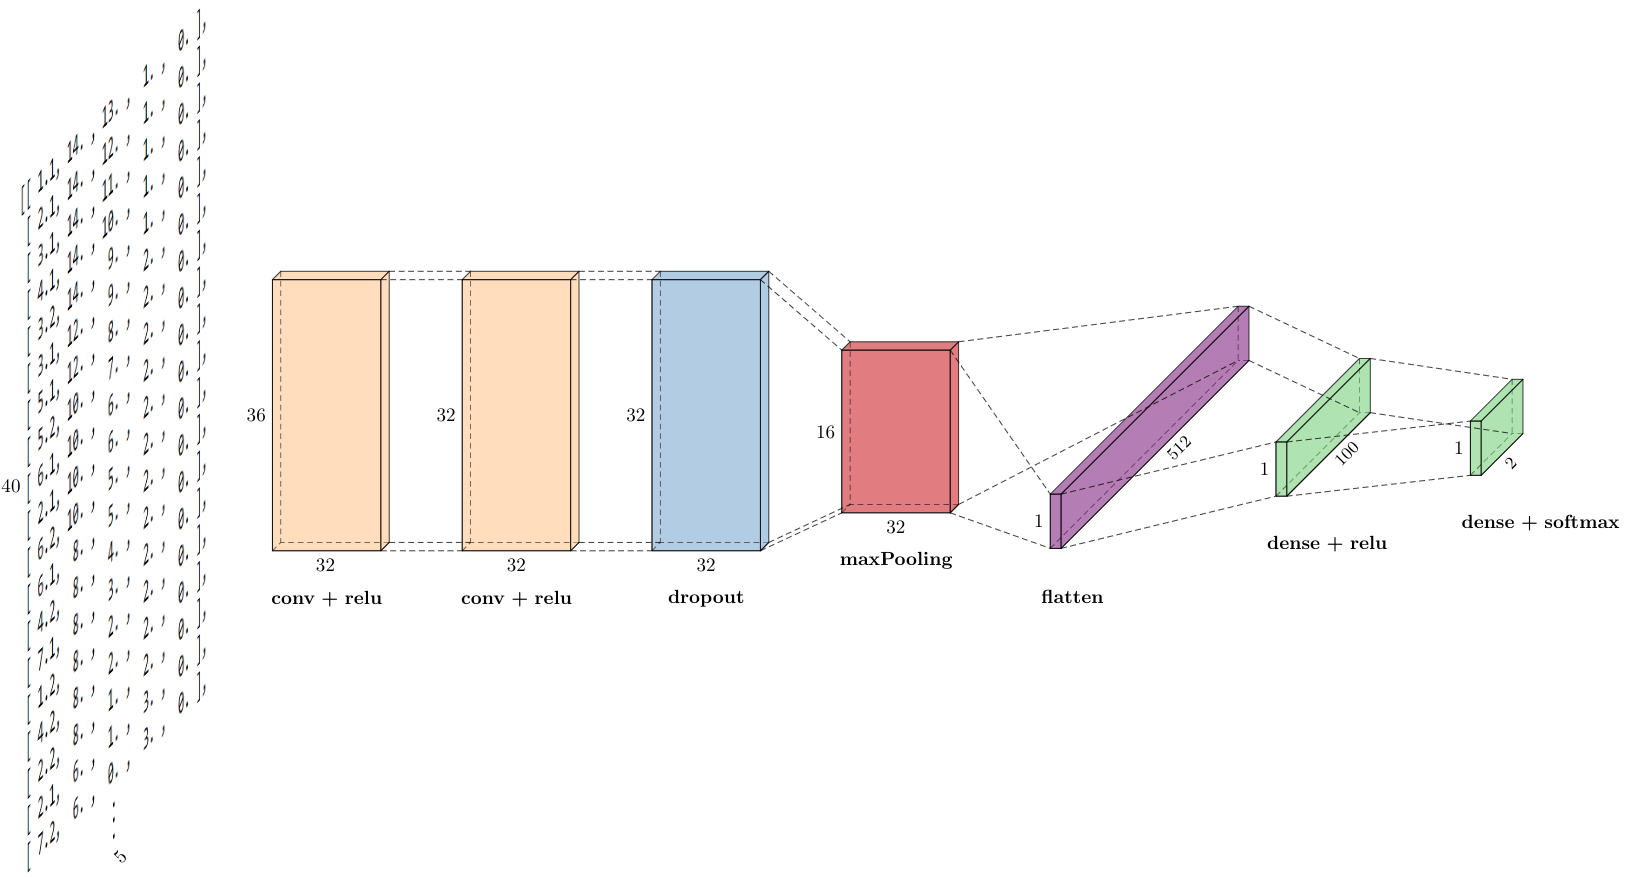
\includegraphics[width=15cm]{images/1dCnnStructureChanged.png}
	\caption[Bild kurz]{The width describes the number of feature maps and the height and depth describe the dimensions of the feature maps. As example after the first convolutional layer the data consists of 32 one dimensional feature maps with the length of 36.}
	\label{fig:1dCnnStructure}
\end{figure}
The input data consist of the 5 statical features, explained in section \todo{ref}, for each of the 40 steps (20 rounds), resulting in the input dimensions 40 $\cdot$ 5. Initially the data is passed to the first convolutional layer of the network. The first layer has 32 filters and the kernel has a size of 5, meaning that every step from the kernel includes all data from 5 steps in the game. Since the input data is two dimensional and the convolution is one dimensional, the created feature maps are one dimensional. Therefore the first convolutional layer creates 32 festure maps each with a size of 36. These feature maps are passed to the second convolutional layer with the same number of filters and the same kernel size as the first layer. This again results in 32 feature maps with a decresed size of 32. Afterwards a dropout layer with a rate of 0.5 randomly sets input units to 0 and by that helps to prevent overfitting. Then a one dimensional max pooling layer with a pool size of 2 reduces the size of the 32 feature maps to 16.  And finally the network is completed with a flatten layer and two dense layers. \todo{vielleicht genauer erklären was dense macht, aber eigentlich ja oben auch schon, nur einen groben satz hier}. Both convolutional layers, and the first dense layer use a rectified linear unit as activation function. The last dense layer uses softmax normalization to bring the data down two two values for the two classes. The elements of the output vector are between 0 and 1 and sum up to 1 and specify the result of the classification. In total 57486 parameters are trained in this model. 

As optimizer the Adam optimizer from keras is used that implements the Adam algorithm. Adam optimization is a stochastic gradient descent method \todo{ref zu keras adam seite}. The learning rate is set to 0.0001 and not changed during the training. The batch size is set to 32 and the model is trained for 2500 epochs. 

\subsection{2D CNN}
The structure of the 1D CNN used is shown in figure \ref{fig:2dCnnStructure}.
\begin{figure}[H]
	\centering
	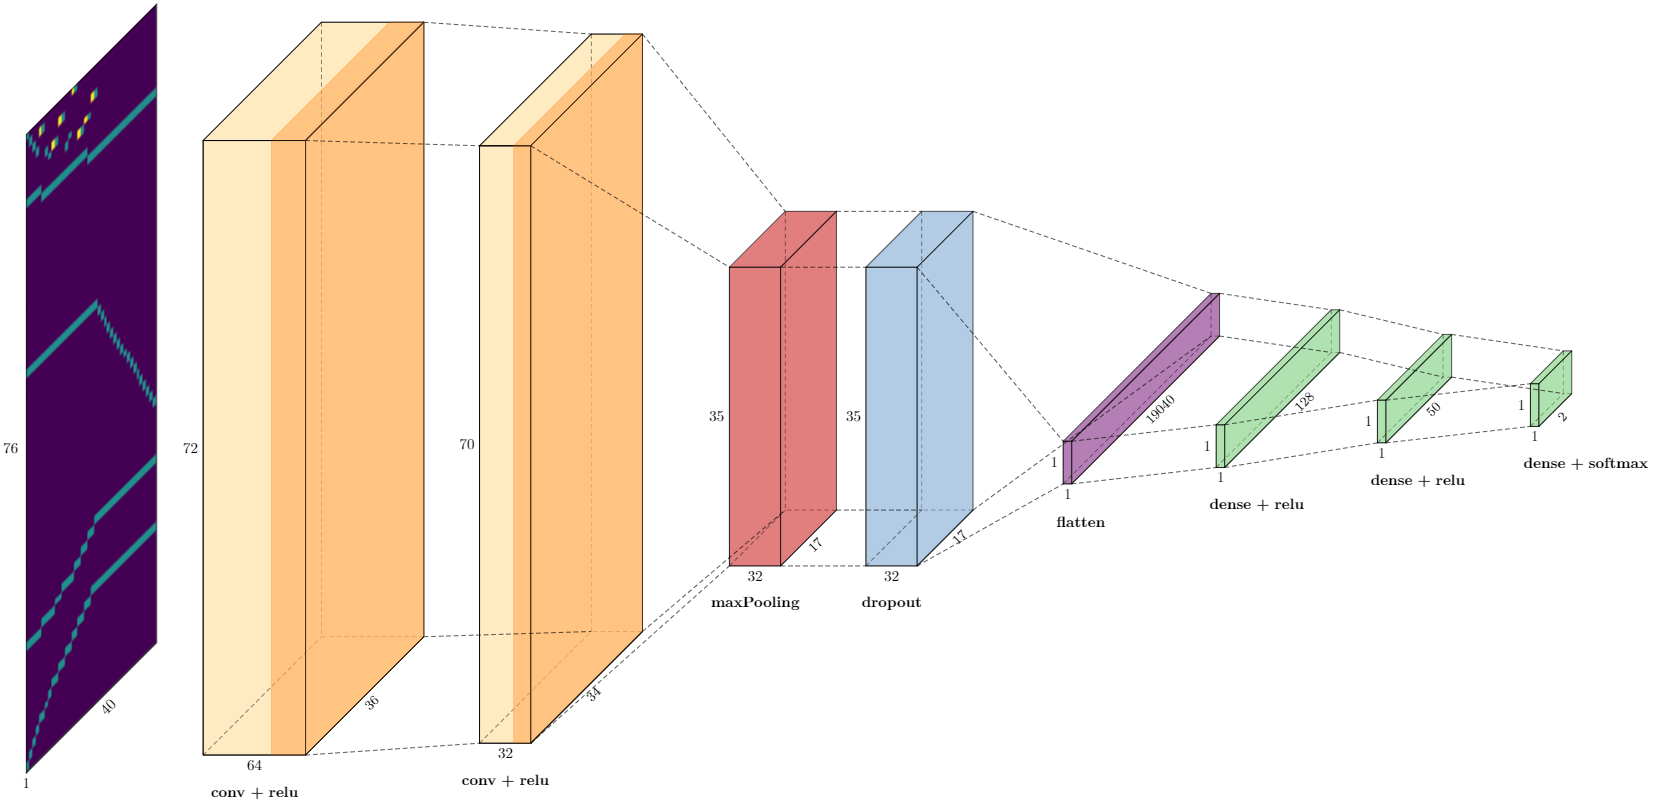
\includegraphics[width=15cm]{images/2dCnnStructure_new.png}
	\caption[Bild kurz]{The width describes the number of feature maps and the height and depth describe the dimensions of the feature maps. As example after the first convolutional layer the data consists of 64 two dimensional feature maps with the size of 72 $\cdot$ 36.}
	\label{fig:2dCnnStructure}
\end{figure}
The input data consist of the synthetic images generated in .. \todo{ref} using the 5 statistical features, resulting in the input dimensions 76 $\cdot$ 40 $\cdot$ 1. Initially the data is passed to the first convolutional layer of the network. The first layer has 64 filters and the kernel has a size of 5 $\cdot$ 5, meaning that each step from the kernel includes a 5 $\cdot$ 5 sized area of the synthetic image. This convolution results in 64 feature maps each with dimensions of 72 $\cdot$ 36. These feature maps are passed to the second convolutional layer with 32 filters and a kernel size of 3 $\cdot$ 3. This results in 32 feature maps and a decresed dimensionality of 70 $\cdot$ 34. Then a two dimensional max pooling layer with a pool size of 2 $\cdot$ 2 reduces the dimensinalty to 35 $\cdot$ 17. Afterwards a dropout layer with a rate of 0.2 randomly sets input units to 0 and by that helps to prevent overfitting. And finally the network is completed with a flatten layer and three dense layers \todo{vielleicht genauer erklären was dense macht, aber eigentlich ja oben auch schon, nur einen groben satz hier}. Both convolutional layers, and the first two dense layers use a rectified linear unit as activation function. The last dense layer uses softmax normalization to bring the data down two two values for the two classes. The elements of the output vector are between 0 and 1 and sum up to 1 and specify the result of the classification. In none of the different operations zero padding was required in order to prevent information loss. In total 2463928 parameters are trained in this model.

As optimizer the Adam optimizer from keras is used that implements the Adam algorithm. Adam optimization is a stochastic gradient descent method \todo{ref zu keras adam seite}. The learning rate is set to 0.00001 and not changed during the training. The batch size is set to 32 and the model is trained for 1000 epochs. 


\begin{comment}

\subsubsection{Visualizing intermediate activations}
\todo{vielleichtz diese section rausnehemen. ich denke es ist unnötig, weil es nicht dazu beiträgt was meine arbeit zeigen soll}

An interesting thing about 2d cnns is that it is possible to vizualize the reprenestations learned by the network. This helps to understand the meaning of individual filters. Intermediate activations canm be vizualized by displaying the feauture maps that are the outpu of various convolution and pooling layers in the network, given an image is passed to the input layer. \todo{ref} To extract these feature maps, the model is first trained for one split and then run in prediction mode. Vizualizing each feature map produced by filters gives a view into how an input is decomposed into the different filters learned by the cnn. The decision was made not to focus too much on vizualizing all feature maps but instead to only vizualize one feature map created by each layer. As each feature map can learn different features, the following visualizations are only small fractions of what the cnn learns. Thgerefore they should only serve as exemplary illustration of what the different layers of the cnn output.

\todo{bisschen beschreiebn was was ist von den bildern und was man sieht}

\begin{minipage}{0.5\textwidth}
\begin{figure}[H]
\centering
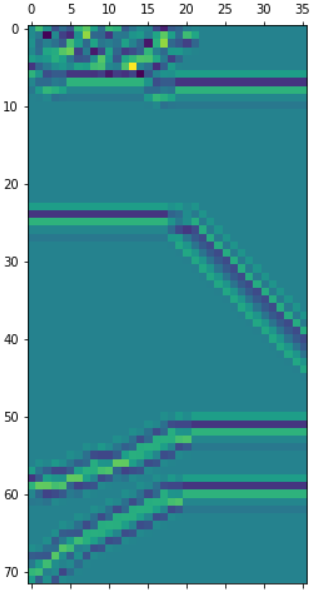
\includegraphics[width=5cm]{images/2dcnnLayer1.png}
\caption[Bild kurz]{Add caption}
\label{fig:vis2d1}
\end{figure}
\end{minipage}
\begin{minipage}{0.5\textwidth}
\begin{figure}[H]
\centering
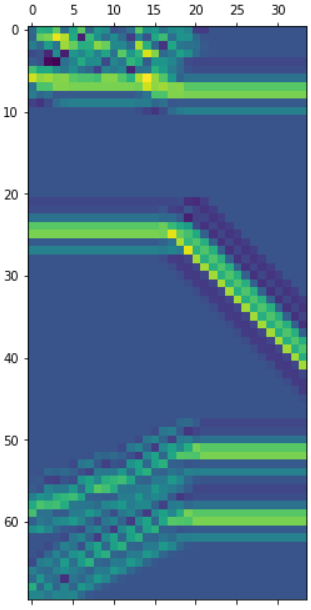
\includegraphics[width=5cm]{images/2dcnnLayer2.png}
\caption[Bild kurz]{Add caption}
\label{fig:vis2d2}
\end{figure}
\end{minipage}

\begin{minipage}{0.5\textwidth}
\begin{figure}[H]
\centering
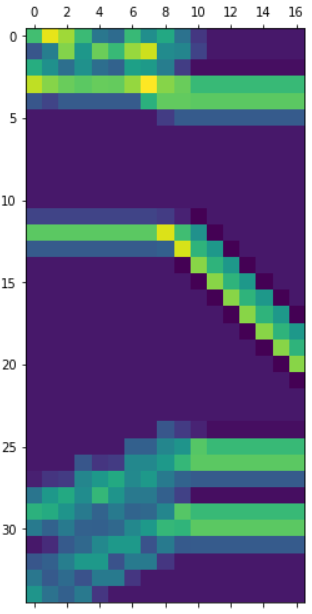
\includegraphics[width=5cm]{images/2dcnnLayer3.png}
\caption[Bild kurz]{Add caption}
\label{fig:vis2d3}
\end{figure}
\end{minipage}
\begin{minipage}{0.5\textwidth}
\begin{figure}[H]
\centering
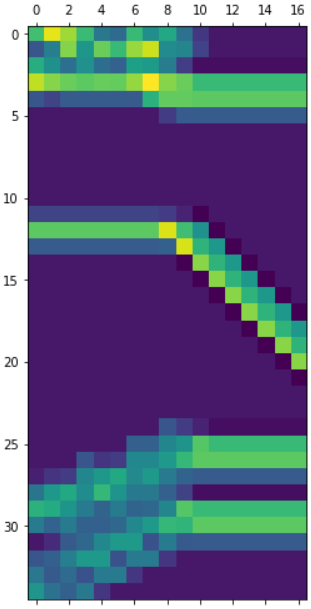
\includegraphics[width=5cm]{images/2dcnnLayer4.png}
\caption[Bild kurz]{Add caption}
\label{fig:vis2d4}
\end{figure}
\end{minipage}

It can be seen that the original structure of the image is still recognizable after all convolutional, pooling and dropout layers. When dealing with cnns that have more layers, usually the original image is at some point not recognizable anymore. The remaining layers of the 2d cnn effectively opperate on one dimensionaml data and create the output. Therfore they will be left out in this vizualization.


%Especially when dealing with more copmplex structures of cnns, vizualizing all feature maps instead of one, can reveal valuable informations. Generelly, the deeper the layer, the less of the original image is recogniazable. Since the size of the 2d cnn used is comparetively small, the original image is still recognizable after all convolutional, poolind and dropout layers.  For instance can be analysed if the structure of the cnn is overly complex for the data. This is the case if the last layers do not activate anymore, as there is nothing more to learn at that point, resulting in all values of the feature maps being 0. 


%If this technique is used for actually analysisng the cnn,  



%An interesting thing about 2d cnns, what is not possible to that extend in most of the neural networks, is that the steps in between can be vizualized. As each convolutional layer creates new images using the filters, it is actually possible to look at the images between layers. Generelly the deeper the layer the less from the actual image is recognizable. It can be observed how the network step by step forms the input image to the output shape. Although this is not especially usefull for actually knowing what the network does, it is usefull for knowing if certain layers of the network do something at all. If for instance the structure of the cnn is overly complex for the data, this will be indicated by the fact that the last layers are not activating at all becuase there is nothing more to learn at that point (all values of all feature maps from a layer are 0). Although the structure of the 2d cnn used is not very complex and this technique is more relevant for larger networks, it is interesting to exemplary look at the images between the convolutions of the 2d cnn used. To do so the model is first trained for one split and then run in predict mode. When passing an image to the imput layer it is then possible to extract the images between layers.

\todo{da wird ein buch erwähnt, wo der typ erzählt wieso es gut ist das zu machen. Die zitate umschreiben in meinen text: \url{https://towardsdatascience.com/visualizing-intermediate-activation-in-convolutional-neural-networks-with-keras-260b36d60d0}}

%... bild..

%As visible, there are no layers from which all filters do not activate, meaning the structure is not overly complex for the data. 

%\todo{referenz finden und bilder einbinden von dem 2d cnn. vielleicht auch ein bild von einem größeren netz wo es nichts mehr lernt.}

\end{comment}

\section{Training setup}
There is one script each for training the 1D cnn and the 2d cnn. The only differences are in the structure and the hyper parameters of the cnns, explained in section \todo{ref}, and that before training the 2d cnn the loaded statistical feaures must first be used to create the synthetic images. Both scripts load the same statistical features, already divided into 20 splits. As there are statistical features for 20 real and 20000 simlauted no obstacles games as well as the same amount for glare effects games, this results in each split containing data from 19 real and 19000 simualted games for each of the two classes, resulting in 38 real and 38000 simulated games available for the training. From 2 real and 2000 simulated games not used for training, only the data from the real games is used for testing. This is done becauuse it is not desirable that the models adapt to the simualted data as in reality they will be only used in real games. Furthermore it can be chosen for which ratios between simualted and real games models should be trained. It was chosen to use ratios of one real game to 0, 1, 2, 3, 4, 5, 6, 7, 8, 9, 10, and 20 simulated games. Moreover it can be chosen how many turns in the game should be used (a turn consists of flipping 2 cards). In real world scenarios, the less the faster the decision is made and assistance can be applied, but if waited the longer the decision will likely be correct more often. To analyse this, models for different amounts of turns are trained. The turns chosen are the first 5, 10, 15 and 20. More than 20 turns were not recorded. \todo{Vielleicht rein: Training models for ranges of turns in the middle, for instance from turn 10 to 15, was left out, because this is not very interesting when conscidering real world usage.} All models are trained twice. Once on the simulated data created before modifying the simulator and once afterwards. This can potentially show whether the changes improved the classification results. 

The structure and hyper parameters of the modells for all 1d cnns are identical. Same goes for all 2d models. The only differnece is the input shape of the modells since it depends on teh number of steps used in the training. Identical structure for modells of the same type are used so that different training results for different amount of steps can be reliably compared. It should be noted the structure and hyper paramters are not the same between the 1d and 2d cnns. 

Once one of the scripts is executed, required directory structures are created and training processes for the different ratios of real to simulated games are performed successively. The training for one ratio consists of parallelized training of 20 splits using multiprocessing. The training for each split is repeated 20 times. As a result for each ratio 20 models are created for every split. This means that 400 models are trained for every ratio. As there are 12 different ratios trained, this results in 4800 models trained for each execution of one of the scripts. As mentioned above, the training is done for 4 different amounts of steps for the 1d cnn and the 2d cnn. This adds up to 38400 models being trained. Furthermore this done twice: Once before the changes to the simulator and once afterwards. All in all this results in 76800 models. For each model the training history is saved in a file. Saving and loading the historeis is neccessary due to the parallel training of multiple models through multiprocessing.  Once the training of the 4800 models of one script is completed, the training histories are loaded from the files. The results from the 400 training histories for each ratio of real to simulated games are averaged, plotted and the final figures are saved for the analysis. The reason for averaging the results over many models is, that deep neural networks by default initialize their weights randomly, resulting in potentially different outcomes of each training. By averaging the results, the values and therefore the interpretation becomes more reliable and meaningful. All models are trained on the cpu. The fact that 76800 models are trained led to the decision, not to save all models but instead first evaluate the results and then retrain and save the models that create the best results. 

\begin{comment}


There are two main folders for storing the classification results. One for the results before the changes to the simulator and the other one for the results afterwards. Once one of the training scripts is executed, a subfolder for saving and loading 
The scripts create and use a specific directory structure conceptualized in figure \todo{ref}.
structure erklären

resutls -> 2d... -> sdxordner,(sdx images) -> split1 -> run1resutls 

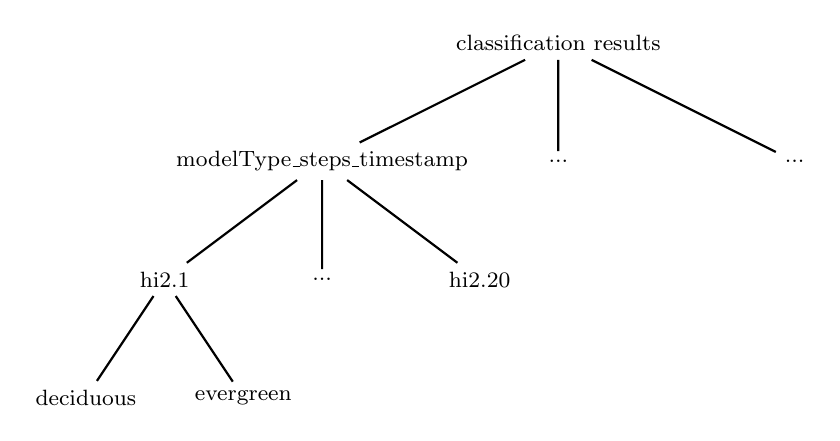
\begin{tikzpicture}
[sibling distance=3cm,-,thick]
\footnotesize
\node {classification results}
child {node {modelType\_steps\_timestamp}
	[sibling distance=2cm]
	child {node {hi2.1}
		child {node {deciduous}}
		child {node {evergreen}}
	}
	child {node {...}}
	child {node {hi2.20}}
}
child {node {...}
}
child {node {...}
}
;
\end{tikzpicture}

\end{comment}

   
\section{Training results and evaluation}
The training results for the various configurations can be seen in table \todo{ref}, \todo{ref}, \todo{ref} and \todo{ref}. The first two tables contain the results before the changes to the simulator and the last to the results afterwards. The analyiss will only focus on the accuracy, but the loss is also listed for the sake of completeness. The best accuracies for each number of turns in each table are highlighted in green. If multiple ratios of real to simulated game for a certain number of turns produce the same accuracy only the one with the smallest amount of simulations is highlighted. The accuracies in the tables are those from the best epochs. In most of the cases the models start overfitting after a certain epoch resulting in a deterioration of the accuracy after reaching a local maximum. All models except the 1d cnns for 5 rounds and ratios of sd0x and sd1x reach such a local maximum in accuracy before the training is stopped. 

It should be claryfied that the chosen configurations of models to be trained make no claim to completeness. The models are not individually optimized and therefore do not neccessarily produce the best results possible. As the amount of collected real data with 20 recordings for each label is very limited, it was decided not to split the data into training, test and validation data, and instead only into training and test data. In order to optimize the models such a validation set would be neccessary. It could be used to tune the hyper parameters of the model. The reason why this is done on a separate validation set is, that the models can then be tested on the test data which was not part of the process of selecting the best hyper parameters. If the models were optimized using the test data, the results would not be representitive of the performance of the models on unknown data. 

\begin{table}[H]
	\centering
	\caption{1D CNN. Best accuracies and losses for 5, 10, 15 and 20 steps. Before the changes to the simulator.}
	\resizebox{\columnwidth}{!}{%
		\begin{tabular}{|c||ccccc|ccccc|ccccc|ccccc|}
			\hline
			&&& 5 r. &&&&& 10 r. &&&&& 15 r. &&&&& 20 r. &&\\
			\hline
			&& Acc. && Loss &&& Acc. && Loss &&& Acc. && Loss &&& Acc. && Loss &\\
			\hline\hline
			sd0x &&     65.12\% && 0.6584 &&& \textcolor{mygreen}{81.12\%} && 0.5116 &&& \textcolor{mygreen}{78.37\%} && 0.5377 &&& 79.62\% && 0.492 &\\
			sd1x &&     71.25\% && 0.6385 &&& 80.88\% && 0.4777 &&& 77.25\% && 0.5355 &&& 80.12\% && 0.4999 &\\
			sd2x &&     68.5\% && 0.6476 &&& 77.38\% && 0.5283 &&& 78.25\% && 0.5275 &&& \textcolor{mygreen}{81.25\%} && 0.4887 &\\
			sd3x &&     69.38\% && 0.6494 &&& 75.5\% && 0.5252 &&& 76.13\% && 0.5329 &&& 79.75\% && 0.4999 &\\
			sd4x &&     67.5\% && 0.6436 &&& 75.88\% && 0.538 &&& 77.25\% && 0.5322 &&& 81.25\% && 0.4975 &\\
			sd5x &&     72.25\% && 0.6212 &&& 76.5\% && 0.5252 &&& 77.75\% && 0.5338 &&& 81.25\% && 0.4985 &\\
			sd6x &&     71.87\% && 0.6346 &&& 74.75\% && 0.547 &&& 76.25\% && 0.5376 &&& 79.38\% && 0.5075 &\\
			sd7x &&     70.25\% && 0.6252 &&& 73.62\% && 0.5395 &&& 76.0\% && 0.5326 &&& 80.0\% && 0.5078 &\\
			sd8x &&     74.25\% && 0.6121 &&& 72.5\% && 0.5509 &&& 77.0\% && 0.535 &&& 79.75\% && 0.4993 &\\
			sd9x &&     \textcolor{mygreen}{74.88\%} && 0.5826 &&& 74.63\% && 0.5483 &&& 76.0\% && 0.542 &&& 81.75\% && 0.4987 &\\
			sd10x &&    74.87\% && 0.5971 &&& 74.5\% && 0.5558 &&& 77.12\% && 0.5394 &&& 80.87\% && 0.5036 &\\
			sd20x &&    73.25\% && 0.5831 &&& 73.5\% && 0.5493 &&& 75.63\% && 0.5355 &&& 80.75\% && 0.5013 &\\
			\hline
		\end{tabular}
	}
\end{table}

\begin{table}[H]
	\centering
	\caption{2D CNN. Best accuracies and losses for 5, 10, 15 and 20 steps. Before the changes to the simulator.}
	\resizebox{\columnwidth}{!}{%
	\begin{tabular}{|c||ccccc|ccccc|ccccc|ccccc|}
		\hline
		&&& 5 r. &&&&& 10 r. &&&&& 15 r. &&&&& 20 r. &&\\
		\hline
		&& Acc. && Loss &&& Acc. && Loss &&& Acc. && Loss &&& Acc. && Loss &\\
		\hline\hline
		sd0x &&     63.5\% && 0.6471 &&& 74.0\% && 0.4991 &&& 79.62\% && 0.4726 &&& 79.0\% && 0.4778 &\\
		sd1x &&     68.12\% && 0.619 &&& 76.62\% && 0.5171 &&& 79.5\% && 0.4984 &&& 81.75\% && 0.4735 &\\
		sd2x &&     68.25\% && 0.6382 &&& \textcolor{mygreen}{80.0\%} && 0.5243 &&& 80.38\% && 0.4851 &&& 84.12\% && 0.4573 &\\
		sd3x &&     69.5\% && 0.6392 &&& 78.88\% && 0.5518 &&& 80.25\% && 0.5038 &&& 84.62\% && 0.4718 &\\
		sd4x &&     67.63\% && 0.6415 &&& 76.38\% && 0.5685 &&& 79.62\% && 0.5106 &&& \textcolor{mygreen}{85.0\%} && 0.4726 &\\
		sd5x &&     70.88\% && 0.6339 &&& 74.63\% && 0.5668 &&& 80.0\% && 0.51 &&& 84.88\% && 0.474 &\\
		sd6x &&     70.62\% && 0.638 &&& 77.0\% && 0.5623 &&& 80.12\% && 0.5077 &&& 84.88\% && 0.4776 &\\
		sd7x &&     69.75\% && 0.6543 &&& 75.38\% && 0.5762 &&& 79.5\% && 0.5176 &&& 85.0\% && 0.4839 &\\
		sd8x &&     70.0\% && 0.6467 &&& 74.25\% && 0.5775 &&& 80.38\% && 0.5164 &&& 85.0\% && 0.484 &\\
		sd9x &&     71.25\% && 0.6395 &&& 78.75\% && 0.5696 &&& \textcolor{mygreen}{81.5\%} && 0.5064 &&& 85.0\% && 0.4814 &\\
		sd10x &&    68.75\% && 0.6296 &&& 77.75\% && 0.5674 &&& 80.12\% && 0.5098 &&& 85.0\% && 0.4802 &\\
		sd20x &&    \textbf{\textcolor{mygreen}{73.0\%}} && 0.5833 &&& 76.63\% && 0.5486 &&& 79.75\% && 0.5064 &&& 84.88\% && 04704 &\\
		\hline
	\end{tabular}
	}
\end{table}

\begin{table}[H]
	\centering
	\caption{1D CNN. Best accuracies and losses for 5, 10, 15 and 20 steps. After the changes to the simulator.}
	\resizebox{\columnwidth}{!}{%
		\begin{tabular}{|c||ccccc|ccccc|ccccc|ccccc|}
			\hline
			 &&& 5 r. &&&&& 10 r. &&&&& 15 r. &&&&& 20 r. &&\\
			\hline
			 && Acc. && Loss &&& Acc. && Loss &&& Acc. && Loss &&& Acc. && Loss &\\
			\hline\hline
			sd0x &&     63.87\% && 0.6698 &&& \textcolor{mygreen}{81.88\%} && 0.5014 &&& 78.5\% && 0.5401 &&& 78.62\% && 0.5107 &\\
			sd1x &&     67.75\% && 0.6648 &&& 79.0\% && 0.5095 &&& 75.75\% && 0.5305 &&& 79.38\% && 0.5101 &\\
			sd2x &&     66.0\% && 0.6506 &&& 79.25\% && 0.4845 &&& 76.0\% && 0.5325 &&& 78.37\% && 0.514 &\\
			sd3x &&     64.38\% && 0.6585 &&& 77.38\% && 0.5037 &&& 77.62\% && 0.5261 &&& 79.25\% && 0.5113 &\\
			sd4x &&     67.0\% && 0.6377 &&& 75.38\% && 0.5289 &&& 77.62\% && 0.5331 &&& \textcolor{mygreen}{80.25\%} && 0.5027 &\\
			sd5x &&     67.0\% && 0.6452 &&& 76.75\% && 0.5146 &&& \textcolor{mygreen}{78.75\%} && 0.5226 &&& 79.0 && 0.5042 &\\
			sd6x &&     70.25\% && 0.6427 &&& 75.25\% && 0.5335 &&& 78.75\% && 0.5208 &&& 79.38\% && 0.5049 &\\
			sd7x &&     70.25\% && 0.6449 &&& 76.88\% && 0.5114 &&& 78.0\% && 0.5129 &&& 78.75\% && 0.5115 &\\
			sd8x &&     71\% && 0.628 &&& 76.25\% && 0.523 &&& 77.25\% && 0.5261 &&& 79.12\% && 0.5156 &\\
			sd9x &&     70\% && 0.6276 &&& 75.37\% && 0.5226 &&& 77.62\% && 0.5281 &&& 78.63\% && 0.522 &\\
			sd10x &&    71.5\% && 0.6242 &&& 76.25\% && 0.5261 &&& 76.38\% && 0.5331 &&& 78.62\% && 0.4986 &\\
			sd20x &&    \textcolor{mygreen}{71.88\%} && 0.6246 &&& 72.38\% && 0.5617 &&& 76.25\% && 0.5416 &&& 79.12\% && 0.5 &\\
			\hline
		\end{tabular}
	}
\end{table}

\begin{table}[H]
	\centering
	\caption{2D CNN. Best accuracies and losses for 5, 10, 15 and 20 steps. After the changes to the simulator.}
	\resizebox{\columnwidth}{!}{%
		\begin{tabular}{|c||ccccc|ccccc|ccccc|ccccc|}
			\hline
			&&& 5 r. &&&&& 10 r. &&&&& 15 r. &&&&& 20 r. &&\\
			\hline
			&& Acc. && Loss &&& Acc. && Loss &&& Acc. && Loss &&& Acc. && Loss &\\
			\hline\hline
			sd0x &&     63.62\% && 0.6461 &&& 73.87\% && 0.4929 &&& 80.0\% && 0.4557 &&& 78.5\% && 0.476 &\\
			sd1x &&     67.88\% && 0.6446 &&& 76.12\% && 0.531 &&& 79.5\% && 0.4911 &&& 79.75\% && 0.4874 &\\
			sd2x &&     69.75\% && 0.6463 &&& \textcolor{mygreen}{79.62\%} && 0.5243 &&& 80.87\% && 0.4905 &&& \textcolor{mygreen}{80.0\%} && 0.4859 &\\
			sd3x &&     69.5\% && 0.6449 &&& 77.5\% && 0.5507 &&& \textcolor{mygreen}{82.25\%} && 0.4994 &&& 80.0\% && 0.4865 &\\
			sd4x &&     69.0\% && 0.6347 &&& 72.75\% && 0.5684 &&& 80.12\% && 0.5156 &&& 80.0\% && 0.495 &\\
			sd5x &&     69.38\% && 0.6342 &&& 73.62\% && 0.5634 &&& 80.5\% && 0.5122 &&& 80.0\% && 0.4917 &\\
			sd6x &&     \textcolor{mygreen}{71.0\%} && 0.6326 &&& 74.5\% && 0.5586 &&& 80.62\% && 0.5038 &&& 79.5\% && 0.4874 &\\
			sd7x &&     70.0\% && 0.6328 &&& 71.62\% && 0.555 &&& 80.0\% && 0.5061 &&& 79.5\% && 0.4874 &\\
			sd8x &&     69.88\% && 0.6287 &&& 72.75\% && 0.5567 &&& 80.25\% && 0.5057 &&& 79.62\% && 0.4874 &\\
			sd9x &&     69.12\% && 0.6238 &&& 72.38\% && 0.5532 &&& 79.5\% && 0.5067 &&& 78.88\% && 0.4887 &\\
			sd10x &&    69.5\% && 0.6203 &&& 73.25\% && 0.5536 &&& 79.5\% && 0.5062 &&& 79.0\% && 0.4904 &\\
			sd20x &&    69.88\% && 0.5935 &&& 73.0\% && 0.5494 &&& 79.62\% && 0.5005 &&& 0\% && 0 &\\
			\hline
		\end{tabular}
	}
\end{table}

\begin{comment}



\begin{table}[H]
	\centering
	\caption{2D CNN. best accuracys for 5, 10, 15 and 20 steps. in brackets behind the accuiracy is the epoch.}%\label{tab1}
	\begin{tabular}{|l|l|l|l|l|}
		\hline
		Simulated Games & 5 steps & 10 steps & 15 steps& 20 steps\\
		\hline
		0 &   & && \\
		1 &  & && \\
		2 &  & && \\
		3 &  & && \\
		4 &  & && \\
		5 & &&& \\
		6 &  & && \\
		7 &  & && \\
		8 &  & && \\
		9 &  & && \\
		10 & &&& \\
		20 & &&& \\
		\hline
	\end{tabular}
\end{table}

\begin{table}[H]
	\centering
	\caption{1D CNN. best accuracys for 5, 10, 15 and 20 steps. in brackets behind the accuiracy is the epoch.}%\label{tab1}
	\begin{tabular}{|l|l|l|l|l|}
		\hline
		Simulated Games & 5 steps & 10 steps & 15 steps& 20 steps\\
		\hline
		0 &   & && \\
		1 &  & && \\
		2 &  & && \\
		3 &  & && \\
		4 &  & && \\
		5 & &&& \\
		6 &  & && \\
		7 &  & && \\
		8 &  & && \\
		9 &  & && \\
		10 & &&& \\
		20 & &&& \\
		\hline
	\end{tabular}
\end{table}

\begin{table}[H]
	\centering
	\caption{2D CNN. 20 turns. config2}%\label{tab1}
	\begin{tabular}{|l|l|l|}
		\hline
		Simulated Games & Best Accuracy (Epoch) & Best Loss (Epoch)\\
		\hline
		0 & 0.7888 (14) & 0.4822 (51) \\
		1 &  &  \\
		2 &  &  \\
		3 &  &  \\
		4 &  &  \\
		5 & 0.8450 (17) & 0.4768 (20) \\
		6 &  &  \\
		7 &  &  \\
		8 &  &  \\
		9 &  &  \\
		10 & 0.8475 (20) & 0.4796 (10) \\
		20 & 0.8437 (6) & 0.4763 (6) \\
		\hline
	\end{tabular}
\end{table}

- 1d cnn können besser mit kurzen sequencen umgehen als 2d. aber 2d sind bei mehr schritten deutlsich besser. (erste einschätzung) 

\begin{table}[H]
	\centering
	\caption{2D CNN. 20 turns. config1}%\label{tab1}
	\begin{tabular}{|l|l|l|}
		\hline
		Simulated Games & Best Accuracy (Epoch) & Best Loss (Epoch)\\
		\hline
		0 & 0.7963 (18) & 0.4931 (98) \\
		1 &  &  \\
		2 &  &  \\
		3 &  &  \\
		4 &  &  \\
		5 & 0.8437 (53) & 0.4821 (31) \\
		6 &  &  \\
		7 &  &  \\
		8 &  &  \\
		9 &  &  \\
		10 &  &  \\
		20 &  &  \\
		\hline
	\end{tabular}
\end{table}

\end{comment}

%- \todo{ich könnte noch plots machen die verlauf entwerder mit festen sd und unterschiedlicher anzahl rounds oder mit feaster rounds und unterscheidlichem sd zeigen. Nicht muss aber wäre cool, falls es sinnvoll ist. Muss ich nochmal gucken. Vielleicht an einem beispeiel um zu zeigen dass es von vorteil sein kann simulierte daten mit zu benutzen in unserem fall}

%- interessant: 1d cnn 5 rounds gucken ob sich der trend weiter führt und sogar noch besser wird

The results show that using a certain number of simulated games for the training can often significantly improve the classificatin resuls over using only the real data. A good example is the accuracy for sd0x compared to sd4x for 20 rounds for the 2d cnn in table \todo{ref}. Using no simulations the accuracy is 79.0\% while for a ratio of 9 simulations for each real game the accuracy is 85.0\%. Furthermore is can be seen that using to many simulations compared to real games can decrease the accuracy. In table \todo{ref}, for 10 rounds, the accuracy for sd2x is 80.0\% and less when using more simulations. This behaviour highly varies depending on the configuration of the model. Sometimes the models produce the best results without any simulations, while other times using simulations strongly outperforms using only real data. It is possible that the optimal ratios of simulated to real games are not included the tested configurations. Especially the 2d cnn for 5 rounds before the changes to the simulator achieves the best accuracy with the highest ratio that was tested. Therefore the optimal ratio could be higher than 20 simulations for each real game. 

When looking at the best accuracies of 1d and 2d cnns for each number of rounds, it can be observed, that the accuracy of the 1d cnns do not get much better and sometimes even worse after more than 10 rounds, while this is not the case for 2d cnns. This can be seen in figure \todo{ref}. The fact that the 1d cnns do not profit from more than 10 rounds might be related to the findings from section \todo{ref}, that indicate that the simulaor perfroms worse in later rounds. However, if the case, this begs the questions why this does not apply to 2d cnns. There is a possibility, that the worse perfromance in later turns has a strong impact on the statistacal features fed to the 1d cnn, but once these feautures are used to create the synthetic images for the 2d cnn this negative impact decreases. Figure \todo{ref} additionally shows the ratios of simulated to real data for each of the best results. The fact that the 2d cnn after 10 rounds still have the best results when using a substantial amount of simulations while the the best results for the 1d cnns after the 10th round use very little simulations, supports the theory from above. Nonetheless the findings are not sufficient to verify the theory. For that more research would be required. However, if found to be true, it could mean that 2d cnns using synthetic images have the potential to handle inacurate simulations better than 1d cnns. From a different perspective, this could also indicate that, assuming the simulator does actually perform worse in later rounds and is improved in that regard, the accuracy of the 1d cnns after 20 rounds could be improved.

\begin{figure}[H]
	\centering
	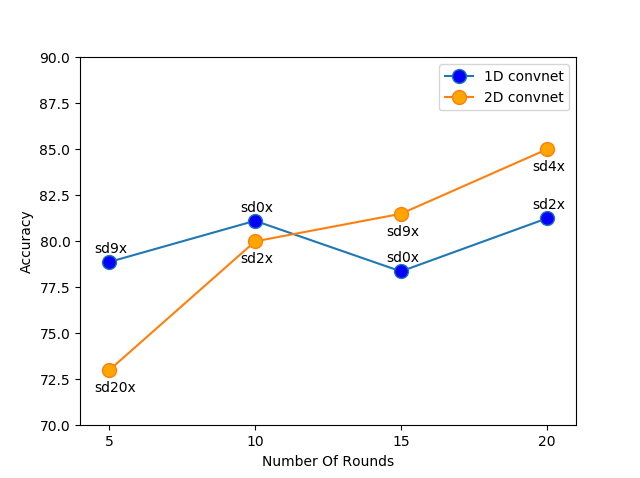
\includegraphics[width=10cm]{images/bestAccPlot.png}
	\caption[Bild kurz]{add caption}
	\label{fig:bestAccPlot}
\end{figure}



%beobachtung: bei 2d sind simulationen länger besser. Analysieren ob es daran liegt dass die anderen keine convergence erreichen. Wenn nicht dann ist es coole entdckung. Weil es ein anzeichen dafür ist, dass die 2d cnn besser mit simulationen lernen kann als 1d cnn. This also fits to the observation, that the results from 1dcnn with more than 10 rounds dont get much better if not worse. This can be caused by the fact that the simulations are less accurate after the first 10 steps, and therefore the 1d cnn does not improve by including them. However, the 2d cnn does improve using the last steps. This is an additional indicator, that the 2d cnn can better handle simulated games. A possibility is, that the difernce between simualted and real games in the synthetic images created using the feautre is not as siificant as when direclty using the statistical features in the 1d cnn. \todo{noch mit zahlen aus den tabelen begründen. und sagen dass die alle convergence erreichen, weshalb man das sagen kann}

% easy to believe that in some cases more the optimal ratio has not been reached yet, if only looking at the tables. However there are more factors that influnece the result. This becomes evident when plotting the trainig histories for accuracy and loss. ... plott wo wan sieht das divergence nicht erreicht wurde... The fact that the trainings with a lower ratio result in worse accuracy dont neccessarily are caused by the fact that more simulated games would be better, but could also be influenced by the fact that the divergence has not been reache yet, meaning that either a different learning rate or more epochs could increase the accuray. Therefore it can not be said with certainty that ore simulated games would in that case lead to the optimal result, as the optimal result could also be with less simulated but with changed hyper parameters. However, the hyper paramaters were intentinally chossen the same so that the results could be compared with each other.
 
It was conscidered to perform statical tests comparing different models and ratios to reveal significant or insignificant differeneces. However, the decision was made that this does not realy gives reliable results, because the values in the tables \todo{ref} are not neccesarily the best accuracies achievable. As mentioned above the models were not individually optimized. Therefoe the results of ststistical tests performed on the achieved accuracies in the tables, would not justify any staements regarding whether 1d cnns or 2d cnns perform significntly better in different configurations. Such statistical test would only show significant differences or indiffierences in the results, but could not be interpreted for any valuable findings, as not all models are used to their full potential. For choosing the best configurations from those tested no statistical tests are used. Instead simply those with the highest accuracies are chosen.

%If hyper paremeters such as the leraning rate or the number of epochs are not chosen equal accross all models of one tabel (menaing all models for 1d cnns, etc) and instead would be chosen more indivuidually to optimize the models specifically for each number of rounds and ratoin between simuated and real games, the accuracie could be signifcantly different. Additionally the topologies of all models of one type are chosen the same, although this might not produce the best results for each configuration.

\begin{table}[H]
	\centering
	\caption{add caption. Upper and lower boundaries are inclusive.}%\label{tab1}
	\resizebox{\columnwidth}{!}{%
		\begin{tabular}{|l||c|c|c|c|c|}
			\hline
			 & 5 r. & 10 r. & 15 r. & 20 r. & Average  \\
			\hline
			\hline
			1D CNN - before & 74.88\% (sd9x) & 81.12\% (sd0x) &78.37\% (sd0x) & 81.25\% (sd2x) & 78.91\% \\
			1D CNN - afterwards& 71.88\% (sd20x) & 81.88\% (sd0x) &78.75\% (sd5x) & 80.25\% (sd4x)  & 78.19\%  \\
			\hline
			2D CNN - before & 73.0\% (sd20x) & 80.0\% (sd2x) &81.5\% (sd9x) & 85.0\% (sd4x)  & 79.88\% \\
			2D CNN - afterwards & 71.0\% (sd6x) & 79.62\% (sd2x) & 82.25\% (sd3x) & 80.0\% (sd2x) & 78.22\% \\
			\hline
		\end{tabular}
	}
\end{table}

Table \todo{ref} shoes the best result for all categories before and after training. It can be seen that although some accuracies are slightly better after the changes to the simulator the results are on average noticeably worse than before. For instance is the accuracy of 85.0\% from the 2d cnn for 20 rounds decreased to 80.0\%. The reason for this is unknown and can be highly complex, due to the many factors involved. A theory is, that reucing the randomness of the simulator and therefore making the simulated games more similar to the real games, may have resulted in decreased generalisation in the models and therefore less robustness on unknown data. However, this theory can hardly be varified. The descreased performce after the changes leads to the decision to only use the models trained on the simulated data created before the changes to the simulator. The chosen configurations can be seen in table \todo{ref}. 

\begin{table}[H]
	\centering
	\caption{add caption. Upper and lower boundaries are inclusive.}%\label{tab1}
	%\resizebox{\columnwidth}{!}{%
		\begin{tabular}{|l||c|c|c|c|}
			\hline
			& 5 r. & 10 r. & 15 r. & 20 r.  \\
			\hline
			\hline
			1D CNN & 74.88\% (sd9x) & 81.12\% (sd0x) & &  \\
			\hline
			2D CNN &  & & 81.5\% (sd9x) & 85.0\% (sd4x)  \\
			\hline
		\end{tabular}
	%}
\end{table}

The 1dnns trained, perform better for 5 and 10 rounds than 2d cnns while 2d cnns perform better for 15 and 12 rounds. Depending on the number of rounds it can therefore be benefitial to use either 1d cnns or 2d cnns. The 4 best configurations for the differnet numbers of rounds are used in section \todo{ref zu voting}. Figures \todo{ref}, \todo{ref}, \todo{ref} and \todo{ref} show the training and test accurcy during the course of training these 4 models. 

\begin{minipage}{0.5\textwidth}
	\begin{figure}[H]
		\centering
		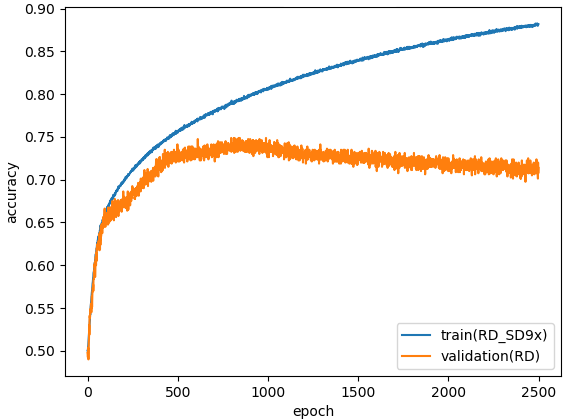
\includegraphics[width=8cm]{images/bestHistories/1d_10s_sd9x_acc.png}
		\caption[Bild kurz]{Add caption}
		\label{fig:1d10}
	\end{figure}
\end{minipage}
\begin{minipage}{0.5\textwidth}
	\begin{figure}[H]
		\centering
		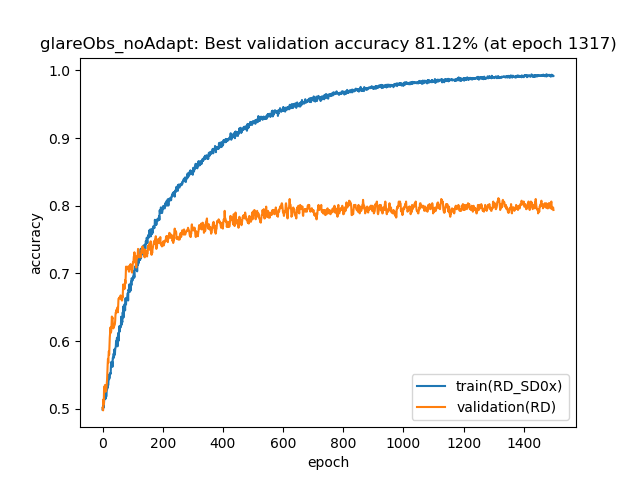
\includegraphics[width=8cm]{images/bestHistories/1d_20s_sd0x_acc.png}
		\caption[Bild kurz]{Add caption}
		\label{fig:1d20}
	\end{figure}
\end{minipage}

\begin{minipage}{0.5\textwidth}
	\begin{figure}[H]
		\centering
		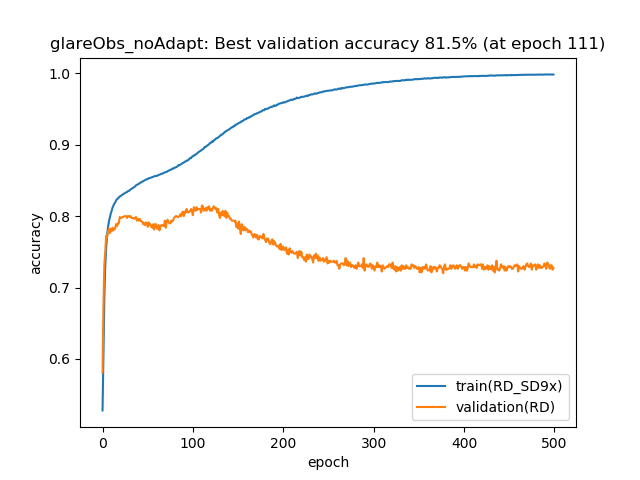
\includegraphics[width=8cm]{images/bestHistories/2d_30s_sd9x_acc.png}
		\caption[Bild kurz]{Add caption}
		\label{fig:2d30}
	\end{figure}
\end{minipage}
\begin{minipage}{0.5\textwidth}
	\begin{figure}[H]
		\centering
		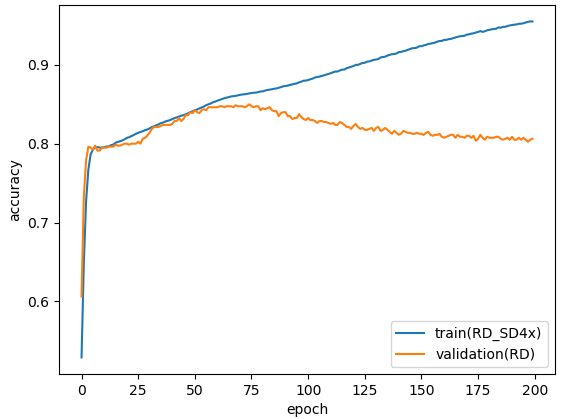
\includegraphics[width=8cm]{images/bestHistories/2d_40s_sd4x_acc.png}
		\caption[Bild kurz]{Add caption}
		\label{fig:2d40}
	\end{figure}
\end{minipage}


%- vielleiht gucken welche falsch erkannt werden und woran es liegt, also wenn die zum beispiel echt schlect oder gut sind obwohl es nicht so sein sollte (rausnhemen und gucken wie ergebnisse sind, vielleicht nur bei bestem modell) -> glaube eher nicht\\
%- training auf welchem rechner/n,was von: cpu oder gpu oder beides, hardware kurz erwähnen, vpn (fernzugriff)\\
%- train test splt, leave one out k fold (+ begründung mit deep learing ..reliable results etc, randomness) \\
%- kurz erklären wieso weniger züge besser sind bei dieser hci erkennung\\
%- (vielleicht kram zu adaptive learning rate ändern und gucken wie es so ist, ansonsten begründen wieso ich das nicht brauche) \\
%- (entweder so dass 1d cnn mit 20 steps auch konvergence erreicht oder danach nochmal anpassung von 20 steps 1d cnn damit es kovergiert)\\
%- darüber schreiben dass letzen n züge nicht mehr so gut simuliert sind (zeigen) und deshalb 40 steps nicht so viel besser ist (glaube nicht dass es so ist, also wahrscheinlich auslassen. Vielleicht bei 15r 1dnn aber man kann es schwer relaible begründen)\\
%- mit maximalen guten steps (glaube 16 züge oder so) trainieren und vergleichen\\
%- statistical tests um signifikante unterschiede /keine unterschiede zu zeigen für verschiedene modelle etc (siehe mazens nachricht) ? \\
